%!TEX root = uist14.tex
\section{IR for head orientation sensing}
\subsection{Hardware}
A central hypothesis of this paper is that the area cursor paradigm~\cite{kabbash1995prince} is well matched to head orientation selection. Head orientation input is imprecise because it does not capture eye movement and has to rely on a low-bandwidth muscle group. Therefore, point selection techniques like laser pointers are not appropriate. 

Infrared emitters are a good technology match since they emit light within a given angle, resulting in a cone in front of the emitter where the light is visible. LEDs with many different fields of view are commercially available. Each individual target that is equipped with IR detector can react to the signal. Such point to point communications enables us to achieve targeting without needing a map.
%% \bjoern{say something about receivers and how point to point connections enable us to leverage head orientation without needing a map.}

Another benefit is the low cost and easy integration of both emitters and detectors - detectors often have support for common IR protocol decoding built in and cost cents, making it economically feasible to add detectors to dozens or hundreds of devices in an environment.

Our augmentation to Google Glass adds a 940nm 5mm IR emitter\footnote{In the prototype, we have used the IR emitter SFH 4545 from OSRAM Opto Semiconductors Inc.} (see Figure~\ref{fig:glass}). \ben{add description about the microcontroller.} In the following description, we refer to Glass because the term is succinct; but other suitable head-worn computing devices could be substituted.

% The IR emitter is the one from OSRAM Opto Semiconductors Inc with manufacturer part number SFH 4545. From the datasheet, it has a view angle of $10^\circ$. Part of the reason we have chosen it is because the radiant intensity can quite high if we provide it with sufficient current flow (550mW/sr @ 100mA). We can then easily adjust it using a resistor to satisfy different demands. 
% % transmitter webpage: http://www.digikey.com/product-search/en?x=0&y=0&lang=en&site=us&KeyWords=475-2919-ND
% For the IR receiver, we use 38.0kHz IR Receiver Modules from Vishay Semiconductor Opto Division (manufacturer part number TSOP38238). 
% % receiver webpage http://www.digikey.com/product-detail/en/TSOP38238/751-1227-ND/1681362
% In order to read the IR intensity, we integrates another IR light-to-voltage converter from AMS-TAOS USA Inc (manufacturer part number TSL267-LF) which is pretty sensitive to IR irradiance. 
% % http://www.digikey.com/product-detail/en/TSL267-LF/TSL267-LF-ND/3095052

While we use IR signal to establish simplex point-to-point communication from Glass to a target, we envision that more complicated applications can be built on top of the selection functionality. Therefore, we added 802.15.4 radios to Glass and all the target nodes to enable bi-directional communication between all nodes and Glass. \bjoern{not entirely correct - we also need node-to-glass communication for the Intensity IR technique.}

\begin{figure}[t]
\centering
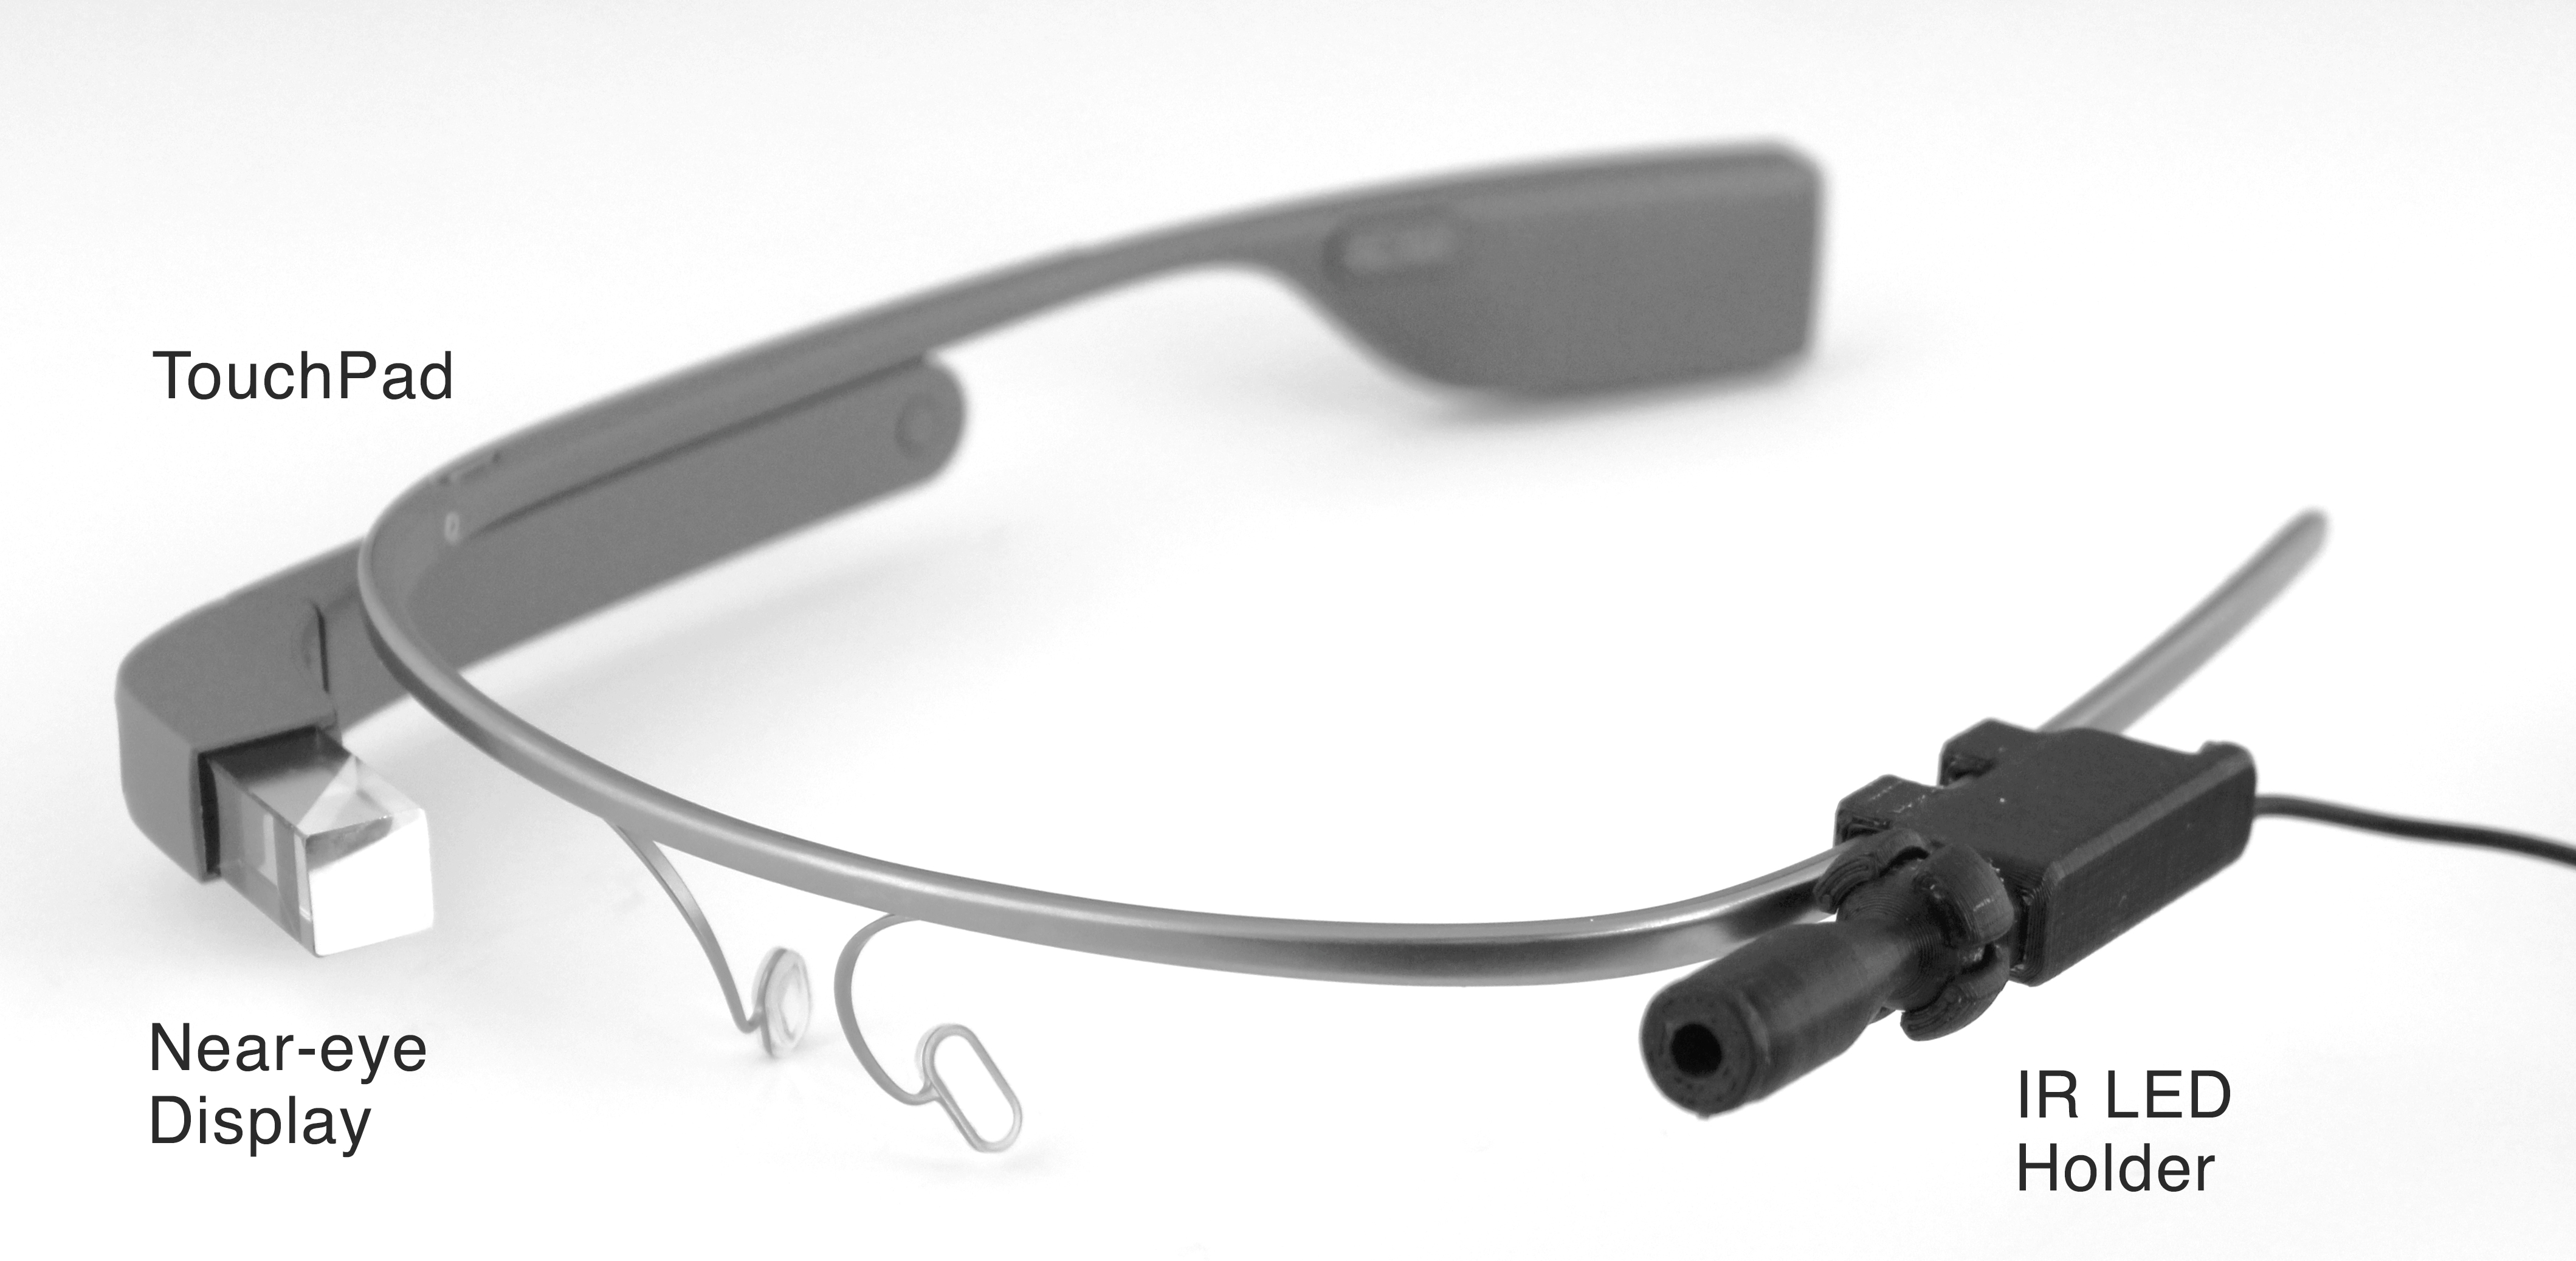
\includegraphics[width=0.9\columnwidth]{figures/GlassWithHolder.jpg}
\caption{Google Glass augmented with a repositionable IR holder.}
\label{fig:glass}
\end{figure}

\subsection{Interaction Model}
From the user's perspective, interaction with \systemname proceeds in two stages (Figure~\ref{fig:interaction}): 

{\bf Scan:} The user first scans the environment to locate the position of the target. During this stage, Glass constantly sends out IR signals, and  targets offer immediate feedback when they receive a signal. The user confirms his desire to connect to a target by tapping on the Glass touchpad. Glass collects the responses from targets that have received IR reception (we use an XBee-based backchannel for this traffic). If there is only one single target in IR range, it is automatically selected. However, in a dense environment where multiple targets are within range, the user needs to perform a refinement.

{\bf Refine:} When disambiguation is needed, the user needs to make an explicit selection among the targets that within his view range. We have designed multiple refinement mechanisms -- all enable the user to select one from a subset of targets. The user confirms a current selection a tap. Since the purpose of this stage is to disambiguate among potential targets, we will also use {\em disambiguation} to refer to this stage. Again, a tap confirms a selection.

\begin{figure}[t!]
\centering
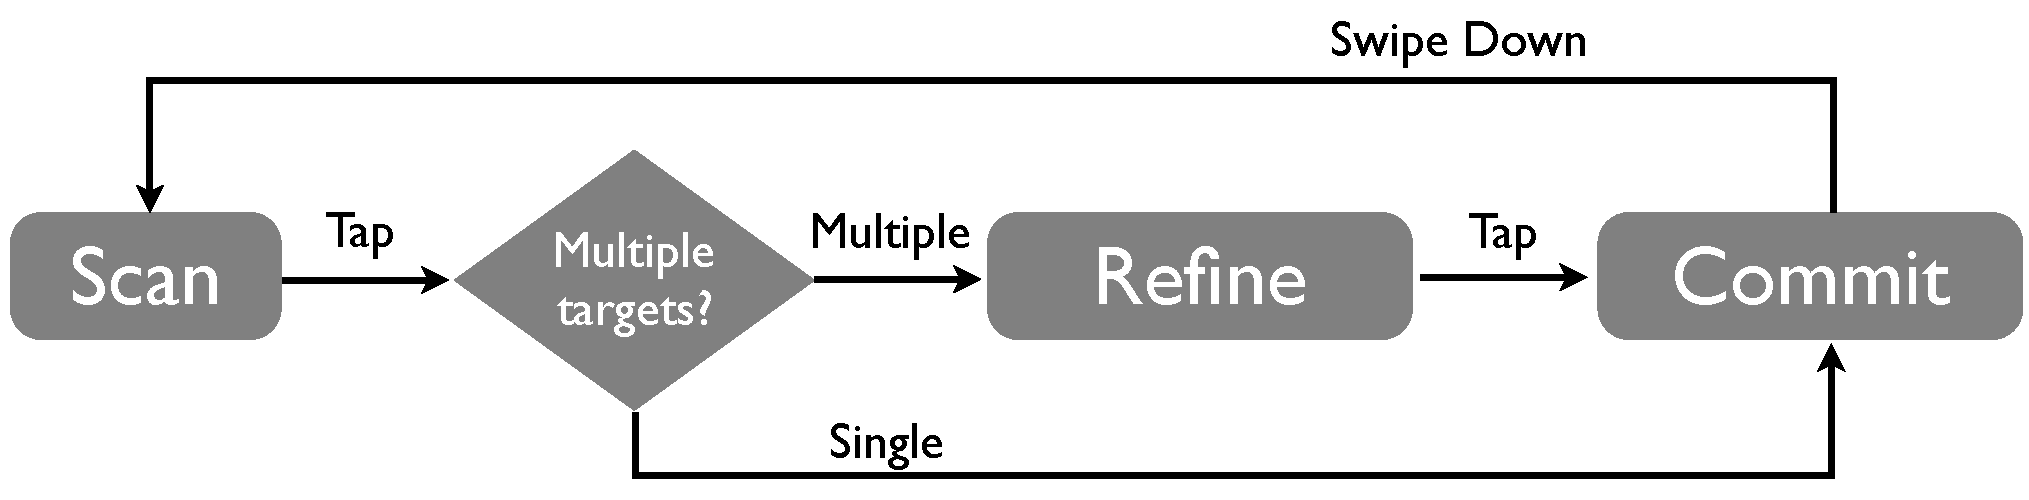
\includegraphics[width=\columnwidth]{figures/interactionModel2.pdf}
\caption{Four different states during the head-orientation targeting.}
\label{fig:interaction}
\end{figure}

The overall target acquisition time thus depends on scan and refine times; the probability that refinement is needed; and the time to commit an action (tap):
\begin{equation}
t_{total}=t_{scan}+P(refine)*t_{refine}+t_{commit}
\end{equation}

In the following sections, we describe our iterative design and evaluation process to minimize the overall target selection time.

%%% Local Variables: 
%%% mode: latex
%%% TeX-master: "uist14"
%%% End: 
